% *********************************************************************
% © 2016–2024 Jeremy Sylvestre
%
% Permission is granted to copy, distribute and/or modify this document
% under the terms of the GNU Free Documentation License, Version 1.3 or
% any later version published by the Free Software Foundation; with no
% Invariant Sections, no Front-Cover Texts, and no Back-Cover Texts. A
% copy of the license is included in the appendix entitled “GNU Free
% Documentation License” that appears in the output document of this
% PreTeXt source code. All trademarks™ are the registered® marks of
% their respective owners.
%
% *********************************************************************
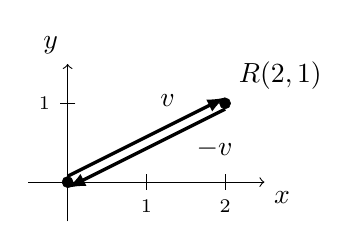
\begin{tikzpicture}[
	point/.style={circle,draw,very thin,fill,inner sep=0pt,minimum size=4pt},
	vector/.style={-latex},
]
	\draw[->] (-0.5,0) to (2.5,0) node[below right] {$x$};
	\draw[->] (0,-0.5) to (0,1.5) node[above left] {$y$};

	\foreach \x in {1,2} {
		\draw (\x,0.1) to (\x,-0.1) node[below] {$\scriptstyle \x$};
	}
	\foreach \y in {1} {
		\draw (0.1,\y) to (-0.1,\y) node[left] {$\scriptstyle \y$};
	}

	\node[point] at (0,0) (o) {};
	\node[point] at (2,1) (r) [label=above right:{$R(2,1)$}] {};
	\draw[vector,very thick] (o.north) to node[above left,near end] {$\uvec{v}$} (r.north);
	\draw[vector,very thick] (r.south) to node[below right, near start] {$-\uvec{v}$} (o.south);

\end{tikzpicture}
